\documentclass{article}
\usepackage{graphicx} % Required for inserting images
\usepackage{algorithm}
\usepackage{algpseudocode}
\usepackage{amsmath}
\usepackage{amssymb}
\usepackage{tikz}
\usepackage{xcolor}
\usepackage{parskip}
\usepackage{hyperref}
\hypersetup{
    colorlinks=true,
    linkcolor=blue,
    filecolor=magenta,      
    urlcolor=blue,
    pdftitle={Overleaf Example},
    pdfpagemode=FullScreen,
    }
\newtheorem{theorem}{Theorem}[section]
\newtheorem{corollary}{Corollary}[theorem]
\newtheorem{lemma}[theorem]{Lemma}

\title{\textbf{Foundation of Machine Learning}}
\author{Lecture : \textbf{Prof. ATIF Jamal} \\ Scribed by : \textbf{HUANG Michel - MEGUENI Samy}}
\date{March 14, 2024}

\begin{document}

\maketitle
\tableofcontents
\vspace{5mm}

\section{Introduction}

\par Previously, we saw the \textbf{Expectation Maximization (EM)} algorithm: allowing to learn distribution among classes thanks to the Latent Variables. Each $x_i$ (observation) is associated to a $z_i$ (latent class).
 
If we succeed in representing the latent space, we're able to generate new data from this space.
\\

From a set of documents, we tried to understand the semantic of their words by using the \textbf{Latent Semantic Analysis (LSA)}. Using LSA, we visualized latent spaces and captured the semantic of each word.
\\

But in reality, even if words are not available in the same document, they can be strongly related.
We need a way to deduce that 2 words are related despite being from different sources: this is where the \textbf{Singular Value Decomposition (SVD)} comes in play.

\section{A concrete case of Singular Value Decomposition (SVD) : Movie Recommendation}
\subsection{Example 1}

\begin{table}[hb]
    \centering
    \begin{tabular}{|c|c|c|c|c|c|}
        \hline
        \textbf{} & \textbf{Matrix} & \textbf{Alien} & \textbf{Star Wars} & \textbf{Casablanca} & \textbf{Titanic} \\
        \hline
        $id_1$ & 1 & 1 & 1 & 0 & 0\\
        $id_2$ & 3 & 3 & 3 & 0 & 0\\
        $id_3$ & 4 & 4 & 4 & 0 & 0\\
        $id_4$ & 5 & 5 & 5 & 0 & 0\\
        $id_5$ & 0 & 0 & 0 & 4 & 4\\
        $id_6$ & 0 & 0 & 0 & 5 & 5\\
        $id_7$ & 0 & 0 & 0 & 2 & 2\\
        \hline
    \end{tabular}
    \caption{Ratings given by users (example 1)}
    \label{tab:ratings_users_1}
\end{table}

We dispose of the following data X (Table~\ref{tab:ratings_users_1}) representing ratings given by users for 5 movies. 
The matrix rank is 2, so we can assume that 2 concepts can emerge from the data : Sci-Fi and Romance movies. \\

\begin{table}[hb]
    \centering
    \begin{tabular}{cccc}
        $\begin{bmatrix}
            1 & 1 & 1 & 0 & 0\\
            3 & 3 & 3 & 0 & 0\\
            4 & 4 & 4 & 0 & 0\\
            5 & 5 & 5 & 0 & 0\\
            0 & 0 & 0 & 4 & 4\\
            0 & 0 & 0 & 5 & 5\\
            0 & 0 & 0 & 2 & 2\\
        \end{bmatrix}$ &
        $=$ &
        $\begin{bmatrix}
            0.14 & 0\\
            0.42 & 0\\
            0.56 & 0\\
            0.70 & 0\\
            0 & 0.60\\
            0 & 0.75\\
            0 & 0.30\\
        \end{bmatrix}$ &
        $\begin{bmatrix}
            12.4 & 0\\
            0 & 9.5\\
        \end{bmatrix}$
        $\begin{bmatrix}
            0.58 & 0.58 & 0.58 & 0 & 0\\
            0 & 0 & 0 & 0.71 & 0.71\\
        \end{bmatrix}$
    \end{tabular}
    \caption{Compact SVD of X}
    \label{tab:decomposition}
\end{table}

Such decomposition is called Compact SVD because the matrix rank is 2 and the remaining 3 singular values are zeros which we don't represent in the decomposition. \\
We're interested in interpreting these spaces.

Let's take a look at each element of the decomposition in Table~\ref{tab:decomposition}:

\[
X = U \Sigma V^{t}
\]

\begin{itemize}
\item $U = \begin{bmatrix} 0.14 & 0 \\ ... & ... \\ 0 & 0.30\\ \end{bmatrix}$ :
    Users x concepts matrix $U \in \mathbb{R}^{u \times c}$
    \\
    
    The first line $\begin{bmatrix} 0.14 & 0\\\end{bmatrix}$ represents the first user.
    He's only represented in the Sci-Fi dimension.
At the difference, the last user described by $\begin{bmatrix} 0 & 0.30\\ \end{bmatrix}$ is only represented by the Romance dimension. \\

    We then have the following space representation in $\mathbb{R}^{u \times c}$:
\begin{center}
\begin{tikzpicture} [scale=0.8]
  % Axes
  \draw[->] (0,0) -- (4,0) node[right] {Sci-Fi};
  \draw[->] (0,0) -- (0,4) node[above] {Romance};
  % Vector
  \draw[->, thick] (0,0) -- (1,0) node[below] {User 1};
  \draw[->, thick] (0,0) -- (0,2) node[left] {User 7};
\end{tikzpicture}
\end{center}

\item $\Sigma = \begin{bmatrix} 12.4 & 0 \\ 0 & 9.5 \\ \end{bmatrix}$ :
    Singular value matrix $\Sigma \in \mathbb{R}^{c \times c}$ \\
    
    $12.4 > 9.5$, which means the Sci-Fi concept weights more than the Romance concept because there are more Sci-Fi movies than Romance one than Romance movies. \\
\item    
 $V^{t}$$ = \[\begin{bmatrix} 0.58 & 0.58 & 0.58 & 0 & 0\\ 0 & 0 & 0 & 0.71 & 0.71\\ \end{bmatrix} : \text{Concepts x products matrix } V^{t} \in \mathbb{R}^{c \times p} \]
    
    The Matrix movie described by the first $\begin{bmatrix} 0.58\\ 0\\\end{bmatrix}$ is only represented by the Sci-Fi dimension. In the same way, the last movie Titanic is only represented by the Romance dimension.\\

    We then have the following space representation in $\mathbb{R}^{c \times p}$:
\begin{center}
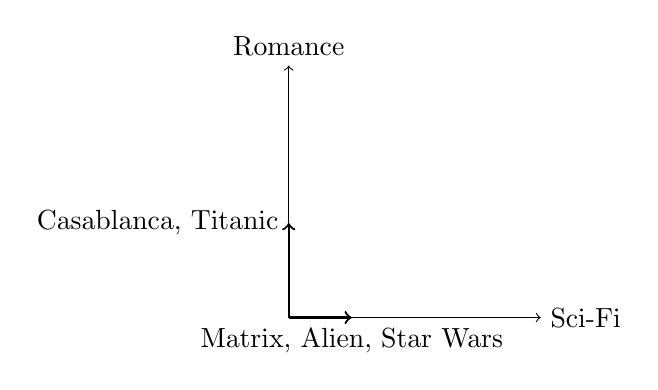
\begin{tikzpicture} [scale=0.8]
  % Axes
  \draw[->] (0,0) -- (4,0) node[right] {Sci-Fi};
  \draw[->] (0,0) -- (0,4) node[above] {Romance};
  % Vector
  \draw[->, thick] (0,0) -- (1,0) node[below] {Matrix, Alien, Star Wars};
  \draw[->, thick] (0,0) -- (0,1.5) node[left] {Casablanca, Titanic};
\end{tikzpicture}
\end{center}
\end{itemize}

Thanks to this decomposition we can represent users and movies in a same sub-space : the space of concepts.\\

We are now able to conceive a recommendation algorithm.

\subsection{Example 2}

Let's see a slightly different table : same as before, but this time users 5 and 7 rated the Alien movie.

\begin{table}[h]
    \centering
    \caption{Ratings given by users (example 2)}
    \label{tab:ratings_users_2}
    \begin{tabular}{|c|c|c|c|c|c|}
        \hline
        \textbf{} & \textbf{Matrix} & \textbf{Alien} & \textbf{Star Wars} & \textbf{Casablanca} & \textbf{Titanic} \\
        \hline
        $id_1$ & 1 & 1 & 1 & 0 & 0\\
        $id_2$ & 3 & 3 & 3 & 0 & 0\\
        $id_3$ & 4 & 4 & 4 & 0 & 0\\
        $id_4$ & 5 & 5 & 5 & 0 & 0\\
        $id_5$ & 0 & 2 & 0 & 4 & 4\\
        $id_6$ & 0 & 0 & 0 & 5 & 5\\
        $id_7$ & 0 & 1 & 0 & 2 & 2\\
        \hline
    \end{tabular}
\end{table}

The matrix rank is not 2 anymore but 3. So we should have 3 different concepts.

But if we take a look at the Singular Value Matrix :

\[
\Sigma = \begin{bmatrix} 12.4 & 0 & 0\\ 0 & 9.5 & 0 \\ 0 & 0 & 1.3 \\ \end{bmatrix}
\]
We now have 3 different singular values but they don't have the same importance.

We can quantify the importance of a concept by dividing its singular value by the sum of all the singular values $Tr(\Sigma)$.

\begin{itemize}
    \item Sci-Fi : $\frac{12.4}{12.4+9.5+1.3} = 0.53$
    \item Romance : $\frac{9.5}{23.2} = 0.41$
    \item Mixed : $\frac{1.3}{23.2} = 0.06$
\end{itemize}

By only picking the first 2 concepts, we keep $94 \%$ of information. \\
We can therefore reduce the dimensions without losing much information. There is a trade-off between dimensionality reduction and information gain, where reducing dimensionality leads to a reduction in information gain, and vice versa. This trade-off is driven by the hyper-parameter k which represents how many singular values we keep in the k-truncated SVD factorization. \\
Using a 2-truncated SVD yields :

\begin{table}[ht]
    \centering
    \begin{tabular}{cccc}
        $\begin{bmatrix}
            0.13 & 0.02\\
            0.41 & 0.07\\
            0.55 & 0.09\\
            0.68 & 0.11\\
            0.15 & -0.59\\
            0.07 & -0.73\\
            0.07 & -0.29\\
        \end{bmatrix}$
        $\begin{bmatrix}
            12.4 & 0\\
            0 & 9.5\\
        \end{bmatrix}$
        $\begin{bmatrix}
            0.56 & 0.59 & 0.56 & 0.09 & 0.09\\
            0.12 & -0.02 & 0.12 & -0.69 & -0.69\\
        \end{bmatrix}$ \\
        = 
        $\begin{bmatrix}
            0.93 & 0.95 & 0.93 & .014 & .014\\
            2.93 & 2.99 & 2.93 & .000 & .000\\
            3.92 & 4.01 & 3.92 & .026 & .026\\
            4.84 & 4.96 & 4.84 & .040 & .040\\
            0.37 & 1.21 & 0.37 & 4.04 & 4.04\\
            0.35 & 0.65 & 0.35 & 4.87 & 4.87\\
            0.16 & 0.57 & 0.16 & 1.98 & 1.98\\
        \end{bmatrix}$
    \end{tabular}
    \caption{Truncated SVD}
    \label{tab:decomposition}
\end{table}

One observes that truncating the SVD yields an approximation $\bar{X}$ of the original matrix X such that $||X-\bar{X}||_F^2$ is as small as possible. Notice that $\bar{X}$ is more dense.

\section{Exercise : 2006 "Netflix Prize" competition}

In 2006, Netflix held the "Netflix Prize" competition, the goal was to predict user ratings based on previous ratings without any other information about the users or films, i.e. without the users being identified except by numbers assigned for the contest. The contest was won in 2009 with a $10\%$ improvement. \\
The solution was to use \href{https://developers.google.com/machine-learning/recommendation/collaborative/matrix}{Matrix Factorization}. \\
Goal : Factorize a rating matrix R into a user x product matrix
Formally, we search for matrices $X \in \mathcal{R}^{n \times c}$ and $Y \in \mathcal{R}^{c \times m}$ such that :

\begin{equation}
    R \approx X Y
\end{equation}
$\cdot$ n is the number of users/observations \\
$\cdot$ m is the number of movies (or items)/the dimension of x \\
$\cdot$ c is the number of concepts/latent dimensions \\
$\cdot$ X maps users to concepts \\
$\cdot$ Y maps concepts to movies \\
$\cdot$ $r_{ui}$ is the rating of user u of the movie i

We also add a regularization term
\begin{equation*}
    min_{X,Y} \ \sum_{u,i} (r_{ui}-x_u^t y_i)^2 + \lambda(\sum_{u=1}^n ||x_u||^2 + \sum_{i=1}^m ||y_i||^2)
\end{equation*}

This is equivalent in matrix notation to:
\begin{equation}
    min_{X,Y} \ ||R-XY||_F^2 + \lambda (||X||_F^2 + ||Y||_F^2) \label{Loss}
\end{equation}
where $||.||_F$ denotes the Frobenius norm for matrices. \\
To solve this equation, we use the alternative least squares (ALS) method :

\begin{algorithm}
\caption{Alternating Least Squares (ALS)}\label{als}
\begin{algorithmic}[1]
\Procedure{ALS}{$R, c, \lambda$}
    \State Initialize matrices $X \in \mathcal{R}^{n \times c}$ and $Y \in \mathcal{R}^{c \times m}$ with random values
    \While{not converged}
        \State Fix $Y$, update $X$:
        \State $X \gets RY^T (YY^T + \lambda I_{c})^{-1}$ \label{line:updateX}
        \State Fix $X$, update $Y$:
        \State $Y \gets (X^TX + \lambda I_{c})^{-1} X^TR$ \label{line:updateY}
    \EndWhile
    \State \textbf{return} $X$, $Y$
\EndProcedure
\end{algorithmic}
\end{algorithm}
where line \ref{line:updateX} and \ref{line:updateY} are obtained by deriving \eqref{Loss} w.r.t X and Y :

\begin{align*}
    \frac{\partial ||R-XY||_F^2 + \lambda (||X||_F^2 + ||Y||_F^2)}{\partial X} &= -2(R-XY)Y^T + 2\lambda X\\
    \frac{\partial ||R-XY||_F^2 + \lambda (||X||_F^2 + ||Y||_F^2)}{\partial Y} &= -2X^T(R-XY) + 2\lambda Y
\end{align*}
Solving for null partial derivative yields :
\begin{align*}
    \frac{\partial ||R-XY||_F^2 + \lambda (||X||_F^2 + ||Y||_F^2)}{\partial X} &= 0_{\mathcal{R}^{n \times c}} \\
    \Longleftrightarrow -2(R-XY)Y^T + 2\lambda X &= 0_{\mathcal{R}^{n \times c}}\\
    \Longleftrightarrow -RY^T +XYY^T + \lambda X &= 0_{\mathcal{R}^{n \times c}} \\
    \Longleftrightarrow X(YY^T + \lambda I_{c}) &= RY^T \\
    \Longleftrightarrow X &= RY^T (YY^T + \lambda I_{c}) \\
    \frac{\partial ||R-XY||_F^2 + \lambda (||X||_F^2 + ||Y||_F^2)}{\partial Y} &= 0_{\mathcal{R}^{n \times c}}\\
    \Longleftrightarrow Y &= (X^TX + \lambda I_{c}) X^TR\\
\end{align*}\\

\section{Random Projection}
Let $\mathcal{S} = \{x_i \in \mathcal{R}^d, i=1,...,n\}$
\begin{lemma}
    Let $k \geq C \epsilon^{-2} log(n)$ \\
    There exists a linear mapping A : $\mathcal{R}^d \longrightarrow \mathcal{R}^k$ with $k \ll d$ such that : 
    \begin{equation*}
        (1-\epsilon) ||x_i-x_j||^2 \leq ||Ax_i - Ax_j||^2 \leq (1+\epsilon)||x_i-x_j||^2
    \end{equation*}
\end{lemma}

The goal of Random Projection is to reduce the dimension of X. The core idea behind it is given in the Johnson-Lindenstrauss lemma, which states that if points in a vector space are of sufficiently high dimension, then they may be projected into a suitable lower-dimensional space in a way which approximately preserves pairwise distances between the points with high probability. \\


\section{Generative Modelling}
We introduce the notion of Probabilistic PCA (cf Bishop Pattern Recognition Machine Learning Book) \\
The idea is to use a probabilistic view of PCA by : \\
- Learning via maximum likelihood \\
- Assuming both latent and observed variables follow a Gaussian distribution

\textbf{Recall : EM algorithm in discrete case}
\begin{align*}
    p(x) = \sum_{k=1}^K \ \pi_k \mathcal{N}(x_i; \mu_k, \Sigma_k)
\end{align*}
\textbf{Continuous latent variable model} \\
\\
Goal : Learn a continuous latent space of dimension p by maximizing the likelihood of the probabilistic model. Here :
\begin{align*}
    p(x_i) = \int_{\mathcal{R}} p(x,z) dz \int_{\mathcal{R}} p(z) p(x|z)dz
\end{align*}
\textbf{Assumptions} : The generative model is as follows 
\begin{equation}
     \ x_i = Wz_i + \mu + \epsilon \ \ \forall i \in \{1,...,n\}
\end{equation}
$\cdot$ $\mu \in \mathcal{R}^d$ is a learned parameter representing a mean \\
$\cdot$ $W \in \mathcal{R}^{d \times p}$ is a learned parameter representing a linear mapping : $\mathcal{R}^d \xrightarrow{} \mathcal{R}^p$ \\
$\cdot$ $\epsilon \in \mathcal{R}^d \sim \mathcal{N}(0,\sigma^2 I)$ is a Gaussian independent noise \\
$\cdot$ z is the continuous latent variables with prior $p(z) \sim \mathcal{N}(0,I)$
\\
\\
With these assumptions, we have : \\
1. The conditional distribution of the observed variable is Gaussian :
\begin{equation*}
    p(x|z) = \mathcal{N}(Wz + \mu, \sigma^2 I)
\end{equation*}
2. The marginal p(x) is also a Gaussian :
\begin{align*}
    p(x) &= \int_\mathcal{R} p(x,z) dz = \int_\mathcal{R} p(x|z)p(z)dz \\
\end{align*}
where
\begin{align*}
    \mathbb{E}[X] &= \mathbb{E}[Wz+\mu+\epsilon] \\
    &= \mathbb{E}[Wz+\mu] + \mathbb{E}[\epsilon] \\
    &= W \times 0_{\mathcal{R}^d} + \mu + 0_{\mathcal{R}^d} \\
    \mathbb{E}[X] &= \mu
\end{align*}
and 
\begin{align*}
    C := Cov(X) &= \mathbb{E}[(X-\mu) (X-\mu)T] \\
    &= \mathbb{E}[(Wz + \mu -\mu + \epsilon) (Wz + \mu -\mu + \epsilon)^T] \\
    &= \mathbb{E}[(Wzz^TW^T) + 2Wz\epsilon + \epsilon\epsilon^T] \\
    &= W\mathbb{E}[zz^T]W^T + 2W\mathbb{E}[z\epsilon^T] + \mathbb{E}[\epsilon\epsilon^T] \\
    &= WI_{d}W^T + 2W \times 0 + \sigma^2 I \\
    C &= WW^T + \sigma^2I
\end{align*}
which means $p(x) \sim \mathcal{N}(\mu,WW^T+\sigma^2I)$























\end{document}
